\documentclass[11pt]{article}
\usepackage[utf8]{inputenc}
\usepackage[T1]{fontenc}
\usepackage{lmodern}
\usepackage{amsmath,amssymb,amsthm}
\usepackage{graphicx}
\usepackage{hyperref}
\usepackage{geometry}
\usepackage{doi}
\geometry{margin=1in}

\input{glyphtounicode}
\pdfgentounicode=1

\newtheorem{theorem}{Theorem}
\newtheorem{proposition}[theorem]{Proposition}
\newtheorem{lemma}[theorem]{Lemma}
\newtheorem{corollary}[theorem]{Corollary}
\newtheorem{definition}{Definition}
\newtheorem{remark}{Remark}

\title{Why Exact Heisenberg Capacity Does Not Determine the Phenomenological Cascade Rate:\\
Observable Heterogeneity, Normalisation, and the Transfer Boundary}

\author{J\'er\^ome Beau}
\date{2026\\Version 1.1}

\begin{document}
  \maketitle

  \begin{abstract}
    O12 gives an exact formula for $\dim W_{\leq n}^{(c)}$, hence for
    $\Sigma_n^{(c)}=\Delta r_n^{(c)}/|S_n|$, and the exact asymptotic capacity exponent $\delta=3$.
    The five reported finite-window slopes $4.42,4.80,4.51,4.27,3.59$ are non-monotone crossover
    statistics, not candidate asymptotic exponents for a capacity-to-rate map.
    We determine which parts of the proposed O7 transfer survive for the exact observable.
    The mean over heterogeneous Weil blocks supplies only a scalar power-law premise.
    A factor $q^{-\eta}$ is constant in any fixed-$q$ regression and changes its intercept, not its
    slope.
    Most decisively, the central coordinate $\gamma$ multiplies each exact Fourier mode by a scalar
    phase and is algebraically invisible to rank, so the proposed central-phase correction vanishes
    identically, $\delta_{\gamma,\mathrm{corr}}=0$.
    Conditional on importing the LPS reciprocal prescription and separately defining an endpoint or
    inter-$q$ estimator, the surviving bookkeeping gives
    \[
      \beta_{\mathrm{diag}} = \frac{1}{\delta_{\mathrm{end}} + \tfrac{1}{2}} + \epsilon(q),
    \]
    where $\delta_{\mathrm{end}}
    =\hat\delta_{\mathrm{exact}}-\eta\log q/\log n^{*}$ and $\epsilon(q)$ remains a modelled
    variance term.
    This is not a native Heisenberg derivation of $\beta^{*}$.
    With the benchmark $\eta=1/2$ and the recorded fitting endpoints, the diagnostic remains below
    $5.0$ at all five primes and selects S2-B.
    \textbf{Interpretive outlook.}
    Exact spectral capacity and a phenomenological cascade rate remain distinct observables until a
    growth carrier and a capacity-to-rate identification are independently constructed.
  \end{abstract}

  \paragraph{Keywords.}
    Heisenberg graphs, exact Weil-block capacity, projective capacity, conditional
    \(\delta \to \beta^*\) prescription, block normalisation, exact rank formula, spectral admissibility,
    central-phase invariance, cross-substrate transfer.

    \clearpage
    \tableofcontents

    \clearpage

  \section{Introduction}
  \label{sec:intro}

  The Cosmochrony framework~\cite{Cosmochrony,Beau2026c} derives particle-physics observables from
  spectral properties of relational graphs associated with binary polyhedral subgroups of
  $\mathrm{SU}(2)$.
  Within the admissibility sub-programme, a central chain of papers---O3
  through O7~\cite{Beau2026a7,Beau2026a8,Beau2026a9,Beau2026a10,Beau2026a11}---proposes, on a
  changing-degree LPS family~\cite{LubotzkyPhillipsSarnak1988}, the relation
  \begin{equation}
    \label{eq:beta_delta}
    \beta^{*} = \frac{1}{\delta + \tfrac{1}{2}},
  \end{equation}
  linking the cascade exponent $\beta^{*}$ to the capacity decay exponent $\delta$.
  Charged-lepton mass ratios constrain $\beta^{*} \in (0.09, 0.13)$~\cite{Beau2026a7}; importing
  \eqref{eq:beta_delta} then induces the target $\delta \in [7.4, 10.6]$.
  The equation is not a native consequence of the fixed-degree Heisenberg Cayley cascade:
  the corpus supplies neither its changing valence nor a growth process carrying the pair
  observable~\cite{Beau2026sgn}.

  Papers O8--O13~\cite{Beau2026a12,Beau2026a13,Beau2026a14,Beau2026a15,Beau2026a16,Beau2026a17}
  develop the computational machinery to measure $\delta$ on Heisenberg graphs
  $G_q = \mathrm{Heis}_3(\mathbb{Z}/q\mathbb{Z})$ via exact Weil-block projective capacity.
  O12 derives the exact asymptotic exponent $\delta=3$ from a closed rank formula.
  O13 reports the finite-window sequence $4.42,4.80,4.51,4.27,3.59$ at
  $q\in\{29,61,101,151,211\}$: it rises from $q=29$ to $q=61$ and then decreases strictly through
  $q=211$.
  These values are crossover statistics approaching the exact exponent, so they cannot support the
  finite-size hypothesis S1 that larger primes drive the asymptotic exponent into $[7.4,10.6]$.

  O13 identifies Source~S2 as an explanation of the tension: the proposed relation
  \eqref{eq:beta_delta} was formulated at the proxy level and does not apply natively to
  the exact Weil-block observable.
  Two surviving gaps separate the exact observable from the imported prescription:
  \begin{enumerate}
    \item \textbf{Normalisation gap.}
    $\Sigma_n^{(c)}$ is normalised by the BFS shell size $|S_n|$, not by the block
    dimension $q$.
    The O7 derivation absorbs this normalisation at the proxy level; its effect in the
    exact-block setting is not derived.
    \item \textbf{Carrier and identification gap.}
    The exact rank formula supplies a capacity observable on fixed-degree Heisenberg graphs.
    It does not supply the changing-degree LPS growth carrier or identify the Heisenberg mean with
    the rate variable entering \eqref{eq:beta_delta}.
  \end{enumerate}

  The present paper resolves the intra-$q$ observable bookkeeping in S2 and records the remaining
  transfer boundary.
  O14 has a single logical target: explaining why the proxy-level prescription
  \eqref{eq:beta_delta} changes class when $\delta$ is replaced by
  $\hat{\delta}_{\mathrm{exact}}$, and separating exact-block identities from conditional
  endpoint and cross-substrate diagnostics.

  \subsection{Position in the O-series}
    \label{sec:position}

    The O-series maps as follows:
    O11 (proxy observable~\cite{Beau2026a15}),
    O12 (exact observable~\cite{Beau2026a16}),
    O13 (asymptotic stability and closure of S1~\cite{Beau2026a17}),
    O14 (present paper: observable bookkeeping and transfer boundary).
    O14 does not add numerical measurements; it supplies the structural theory that was identified
    as missing in O13~\S8.3.

  \subsection{Logical status of the three central objects}
    \label{sec:logical_status}

    Three objects play distinct logical roles throughout this paper, and their hierarchy must
    be kept clear.

    \begin{description}
      \item[$\hat{\delta}_{\mathrm{exact}}$]
      The \emph{finite-window statistic}: the power-law exponent extracted by log-log regression
      from the mean block capacity $\bar{\Sigma}_n$ on $G_q$, as defined and measured in
      O12--O13~\cite{Beau2026a16,Beau2026a17}.
      It is associated with a specific computational procedure (exact Weil projection, BFS on
      $G_q$, and a fitting window satisfying~(E1$'$)--(E3)).
      Its values $\hat{\delta}_{\mathrm{exact}}(q) \in [3.59, 4.80]$ for
      $q \in \{29,61,101,151,211\}$ are inputs to O14, not outputs, and are distinct from the
      exact asymptotic exponent $\delta=3$.

      \item[$\delta_{\mathrm{eff}}$]
      A conditional \emph{endpoint-normalised diagnostic}:
      $\hat{\delta}_{\mathrm{exact}}-\eta\log q/\log n^{*}$.
      It is not the intra-$q$ OLS exponent: multiplication by $q^{-\eta}$ changes the intercept,
      not the slope in $\log n$.
      The normalisation exponent $\eta$ is a \emph{benchmark parameter}: the value $\eta=1/2$ is
      used in the numerical table, but no inter-$q$ estimator or selection theorem derives it
      (open direction O14-O1, Section~\ref{sec:open}).

      \item[$\beta^{*}$]
      The phenomenological cascade parameter entering the mass-ratio
      formula of O3~\cite{Beau2026a7}, constrained phenomenologically to
      $\beta^{*} \in (0.09, 0.13)$.
      It is not directly measured by O14.
      Applying \eqref{eq:beta_corrected} produces only a conditional diagnostic because the
      reciprocal law is imported from the LPS model.
    \end{description}

    The distinction between $\hat{\delta}_{\mathrm{exact}}$ (measured, procedure-dependent) and
    $\delta_{\mathrm{eff}}$ (an endpoint/inter-$q$ diagnostic) is central to O14's interpretation.

  \subsection{Main results}
    \label{sec:results_summary}

    \begin{enumerate}
      \item We exhibit the precise class of observable implicit in the O7 derivation and show it
      differs from the exact-block observable through two surviving gaps
      (Section~\ref{sec:mismatch}).
      \item We prove that the central phase is exactly invisible to the rank observable, so
      $\delta_{\gamma,\mathrm{corr}}=0$
      (Section~\ref{sec:decomposition}).
      \item We separate the exact intra-$q$ slope from the endpoint/inter-$q$ diagnostic and
      state the reciprocal output only under the imported two-substrate hypothesis
      (Section~\ref{sec:corrected_relation}).
      \item We evaluate the surviving endpoint diagnostic numerically and show that
      it selects S2-B
      (Section~\ref{sec:numerical}).
    \end{enumerate}

  \section{Background and Notation}
  \label{sec:background}

  \subsection{Heisenberg graph and Weil blocks}
    \label{sec:heis}

    Fix an odd prime $q$.
    The Heisenberg group $G_q = \mathrm{Heis}_3(\mathbb{Z}/q\mathbb{Z})$ has order $q^3$ and centre
    $Z(G_q) \cong \mathbb{Z}/q\mathbb{Z}$.
    An element is written $(a,b,\gamma)$ with $a,b \in \mathbb{Z}/q\mathbb{Z}$ and
    $\gamma \in \mathbb{Z}/q\mathbb{Z}$.
    The $q-1$ faithful irreducible representations $\rho_j$, with
    $j\in(\mathbb{Z}/q\mathbb{Z})^{\times}$, each have dimension $q$; the finite-field
    Stone--von Neumann and Weil framework is reviewed in~\cite{GurevichHadani2009}.
    The three-fold tensor product used by the fingerprint construction decomposes into blocks
    $H_c$ indexed by multi-indices $c=(c_1,c_2,c_3)$.
    A block is generic when $c_i\neq0$ and $A=c_1+c_2+c_3\neq0\bmod q$; every generic block has
    dimension $q$~\cite{Beau2026a16}.
    The \emph{block-level projective capacity} at BFS depth $n$ is
    \begin{equation}
      \label{eq:sigma_def}
      \Sigma_n^{(c)} = \frac{\Delta r_n^{(c)}}{|S_n|},
    \end{equation}
    where $\Delta r_n^{(c)}$ is the incremental projective span in $H_c$ and
    $|S_n|$ is the BFS shell size at depth $n$.
    The mean over blocks is $\bar{\Sigma}_n = \mathbb{E}_c[\Sigma_n^{(c)}]$.

  \subsection{Proxy-level capacity and the O7 derivation}
    \label{sec:o7}

    The O7 derivation~\cite{Beau2026a11} operates on a \emph{scalar global capacity}
    $C_n^{\mathrm{proxy}}$, defined via a Fourier-character proxy that abelianises the representation
    structure.
    The derivation yields \eqref{eq:beta_delta} under three implicit assumptions:
    \begin{enumerate}
      \item[(A1)] The observable is a \emph{scalar} function of BFS depth $n$, independent of the
      representation label $c$.
      \item[(A2)] The normalisation is \emph{homogeneous}: the only length scale entering the
      normalisation is $|S_n|$.
      \item[(A3)] There is no \emph{internal structure} within the observable: no block dimension $q$
      and no projective-frequency geometry within a block.
    \end{enumerate}

    These assumptions describe the scalar proxy of O11~\cite{Beau2026a15}.
    For the exact Weil observable measured in O12--O13~\cite{Beau2026a16,Beau2026a17}, block
    heterogeneity and projective-frequency overlap must be retained explicitly.
    The central coordinate is not an additional mismatch term because it is exactly invisible to rank.

  \section{Observable-Class Mismatch}
  \label{sec:mismatch}

  \subsection{Failure of assumption (A1): block heterogeneity}
    \label{sec:a1}

    For the exact Weil observable, $\Sigma_n^{(c)}$ varies across blocks $c$ at fixed $n$.
    O12 Table~2 and O13 Table~3~\cite{Beau2026a16,Beau2026a17} show that condition (E2), which
    requires block-by-block universality, is violated at $q \in \{29,53,61\}$ and satisfied only at
    $q \in \{101,151,211\}$ after the representation variety has been sufficiently sampled.

    Consequently, $\hat{\delta}_{\mathrm{exact}}$ is a property of the \emph{mean}
    $\bar{\Sigma}_n$, not of an individual scalar observable.
    The O7 argument operates on the latter; its extension to the former supplies only the scalar
    power-law premise and leaves the growth-model premises separate.

    \begin{proposition}[Scope of mean universality]
      \label{prop:mean_universality}
      Suppose $\bar{\Sigma}_n \sim C_0 \, n^{-\delta_{\mathrm{eff}}}$ holds with $R^2 \geq 0.97$ over
      a fitting window satisfying condition~(E1$'$).
      Then the mean has a well-defined finite-window decay exponent.
      This discharges only the scalar power-law premise of the O7 argument.
      It does not supply the changing-degree growth equation, the multiplicative coupling of
      redundancy to its productive frontier, or the identification of the Heisenberg mean with
      the LPS capacity variable.
    \end{proposition}

    \begin{proof}
      The assumed fit supplies the stated exponent for $\bar{\Sigma}_n$ by definition.
      The remaining premises concern a distinct growth model and do not follow from mean
      universality~\cite{Beau2026sgn}.
    \end{proof}

  \subsection{Failure of assumption (A2): normalisation by block dimension}
    \label{sec:a2}

    Every generic block $H_c$ has internal dimension $q$.
    The incremental span $\Delta r_n^{(c)}$ accumulates in that $q$-dimensional space.
    The normalisation in \eqref{eq:sigma_def} divides by $|S_n|$ (graph-level shell size) but not
    by $q$.

    \begin{definition}[Amplitude-renormalised observable]
      \label{def:block_normalised}
      For an explicitly chosen exponent $\eta$, define
      \begin{equation}
        \label{eq:sigma_norm}
        \widetilde\Sigma_n^{(c)}=q^{-\eta}\Sigma_n^{(c)}.
      \end{equation}
      This definition does not select $\eta$ or identify an inter-$q$ estimator.
    \end{definition}

    \begin{proposition}[Fixed-$q$ slope invariance]
      \label{prop:fixed_q_invariance}
      At fixed $q$, multiplication of a positive observable by $q^{-\eta}$ leaves every OLS slope
      against $\log n$ unchanged.
      Hence a term $\eta\log q/\log n^{*}$ cannot be subtracted from the intra-$q$ fitted exponent
      $\hat\delta_{\mathrm{exact}}(q)$.
    \end{proposition}

    \begin{proof}
      In logarithmic coordinates,
      $\log(q^{-\eta}\Sigma_n) = \log\Sigma_n-\eta\log q$.
      The second term is constant across the fitting window, so it changes only the regression
      intercept.
      A quotient by $\log n^{*}$ arises only in an endpoint estimator such as
      $-\log\Sigma_{n^{*}}/\log n^{*}$, or in a separately specified inter-$q$ estimator.
    \end{proof}

    The distinction is therefore estimator-dependent.
    The exact observable already fixes the shell normalisation as $|S_n|^{-1}$.
    A factor $q^{-\eta}$ may be useful for comparing amplitudes across primes, but it cannot
    correct an intra-$q$ slope.
    Defining an inter-$q$ estimator and determining $\eta$ for it remain open direction O14-O1
    (Section~\ref{sec:open}).

  \subsection{Assumption (A3): projective-frequency geometry, not central-phase mixing}
    \label{sec:a3}

    In each irreducible factor $\rho_j$, a Heisenberg element $(a,b,\gamma)$ acts by a translation,
    a modulation, and the scalar factor
    \begin{equation}
      \label{eq:phase}
      \psi_j(\gamma + bx) = e^{2\pi i j\gamma/q}\,e^{2\pi i jbx/q}.
    \end{equation}
    The factor involving $\gamma$ is constant in the coordinate $x$.
    Multiplying a non-zero fingerprint vector by this scalar changes neither its projective class nor
    the span rank.
    The internal structure relevant to $\Sigma_n^{(c)}$ is instead the overlap geometry of the
    projective frequencies $(\alpha,\beta)=(B/A,C/A)\bmod q$ in O12's exact rank formula.
    This geometry depends on the visited lateral data and can vary with $c$, producing block
    heterogeneity without any causal contribution from $\gamma$.

  \section{Decomposition of the Exact Observable}
  \label{sec:decomposition}

  \begin{proposition}[Exact central-phase invariance]
    \label{prop:gamma_bias}
    For every odd prime $q$, every faithful block $c$, and every BFS depth $n$, the exact rank
    observable is independent of the central coordinates of the visited elements.
    Consequently,
    \begin{equation}
      \label{eq:gamma_bias}
      \Sigma_n^{\gamma}\equiv0,
      \qquad
      \delta_{\gamma,\mathrm{corr}}=0.
    \end{equation}
  \end{proposition}

  \begin{proof}
    O12's exact rank formula identifies $\dim W_{\leq n}^{(c)}$ with the cardinality of the set of
    projective frequencies $(\alpha,\beta)=(B/A,C/A)\bmod q$ reached by depth $n$.
    The central coordinate appears only through the non-zero scalar
    $e^{2\pi i c\gamma/q}$ multiplying a single Fourier mode.
    Scalar multiplication leaves that mode's projective class and every span dimension unchanged.
    Hence neither $\dim W_{\leq n}^{(c)}$ nor $\Sigma_n^{(c)}$ depends on $\gamma$.
    Any exponent correction attributed to $\gamma$ is therefore exactly zero~\cite{Beau2026a16}.
  \end{proof}

  \begin{remark}
    Shell-level central-coordinate coherence can be computed as a diagnostic of BFS sampling, but it
    is not an input to the rank observable.
    A Weil character-sum bound cannot convert this independent statistic into a rank correction.
  \end{remark}

  \section{Conditional Reciprocal Diagnostic}
  \label{sec:corrected_relation}

  \begin{proposition}[Conditional endpoint diagnostic]
    \label{thm:corrected}
    Assume all of the following:
    (i) the LPS capacity-to-rate prescription \eqref{eq:beta_delta} is imported as a
    cross-substrate hypothesis;
    (ii) $\delta_{\mathrm{eff}}$ is defined by an endpoint or specified inter-$q$ estimator rather
    than the intra-$q$ OLS slope; and
    (iii) the block-variance model used below holds.
    Then the bookkeeping defines the phenomenological diagnostic
    \begin{equation}
      \label{eq:beta_corrected}
      \beta_{\mathrm{diag}}(q)
      = \frac{1}{\delta_{\mathrm{eff}}(q) + \tfrac{1}{2}} + \epsilon(q),
    \end{equation}
    where
    \begin{equation}
      \label{eq:delta_eff}
      \delta_{\mathrm{eff}}(q) = \hat{\delta}_{\mathrm{exact}}(q)
      - \eta \cdot \frac{\log q}{\log n^{*}(q)},
    \end{equation}
    and $\epsilon(q)=O(V_n^{\max}(q))$ is a modelled block-variance term.
    The formula does not identify $\beta_{\mathrm{diag}}$ with the native Heisenberg span-growth
    exponent or establish $\beta^{*}$.
  \end{proposition}

  \begin{proof}
    Under premise~(i), substitution of the endpoint definition \eqref{eq:delta_eff} into the
    imported reciprocal law gives \eqref{eq:beta_corrected}; premise~(iii) appends the stated
    variance term.
    Proposition~\ref{prop:fixed_q_invariance} shows why this is not a correction of the intra-$q$
    regression slope.
    None of these algebraic substitutions supplies a native Heisenberg growth equation.
  \end{proof}

  \begin{remark}
    Equation~\eqref{eq:delta_eff} contains one non-trivial endpoint term.
    Proposition~\ref{prop:gamma_bias} removes the central-phase term algebraically, while
    Proposition~\ref{prop:fixed_q_invariance} shows that $q^{-\eta}$ changes only the intercept of a
    fixed-$q$ regression.
  \end{remark}

  \section{Pipeline Evaluation of the Conditional Diagnostic}
  \label{sec:numerical}

  The companion script \texttt{SpectralO14\_simulation.py} reads the committed O12/O13 pipeline
  files and extracts $\hat\delta_{\mathrm{exact}}$, the fitting endpoint $n_1$, and the shell-level
  central-coordinate coherence.
  The coherence statistic is retained only as a null control: Proposition~\ref{prop:gamma_bias}
  proves that it cannot affect $\Sigma_n^{(c)}$.

  With the explicit benchmark $\eta=1/2$, define
  \begin{equation}
    \label{eq:norm_corr}
    \delta_{\mathrm{end}}(q)=\hat\delta_{\mathrm{exact}}(q)
    -\eta\frac{\log q}{\log n_1(q)}.
  \end{equation}
  The benchmark is a chosen normalisation for this displayed endpoint statistic.
  It is not derived from phase decorrelation and does not define an inter-$q$ estimator.

  \begin{table}[ht]
    \centering
    \caption{Conditional endpoint diagnostic from the O12/O13 pipeline.
      The finite-window slopes are crossover statistics; $\eta=1/2$ is a benchmark, and the exact
      central-phase correction is zero.
      Neither $\delta_{\mathrm{end}}$ nor $\beta_{\mathrm{diag}}$ is a native fitted exponent or a
      derived cascade parameter.}
    \label{tab:endpoint}
    \begin{tabular}{cccccc}
      \hline
      $q$ & $\hat\delta_{\mathrm{exact}}$ & $n_1$ & $\eta\log q/\log n_1$ &
      $\delta_{\mathrm{end}}$ & $\beta_{\mathrm{diag}}$ \\
      \hline
      29  & 4.416 & 5  & 1.0461 & 3.3696 & 0.2584 \\
      61  & 4.799 & 7  & 1.0563 & 3.7423 & 0.2357 \\
      101 & 4.515 & 10 & 1.0022 & 3.5124 & 0.2492 \\
      151 & 4.267 & 12 & 1.0096 & 3.2570 & 0.2662 \\
      211 & 3.588 & 13 & 1.0433 & 2.5452 & 0.3284 \\
      \hline
    \end{tabular}
  \end{table}

  \begin{figure}[ht]
    \centering
    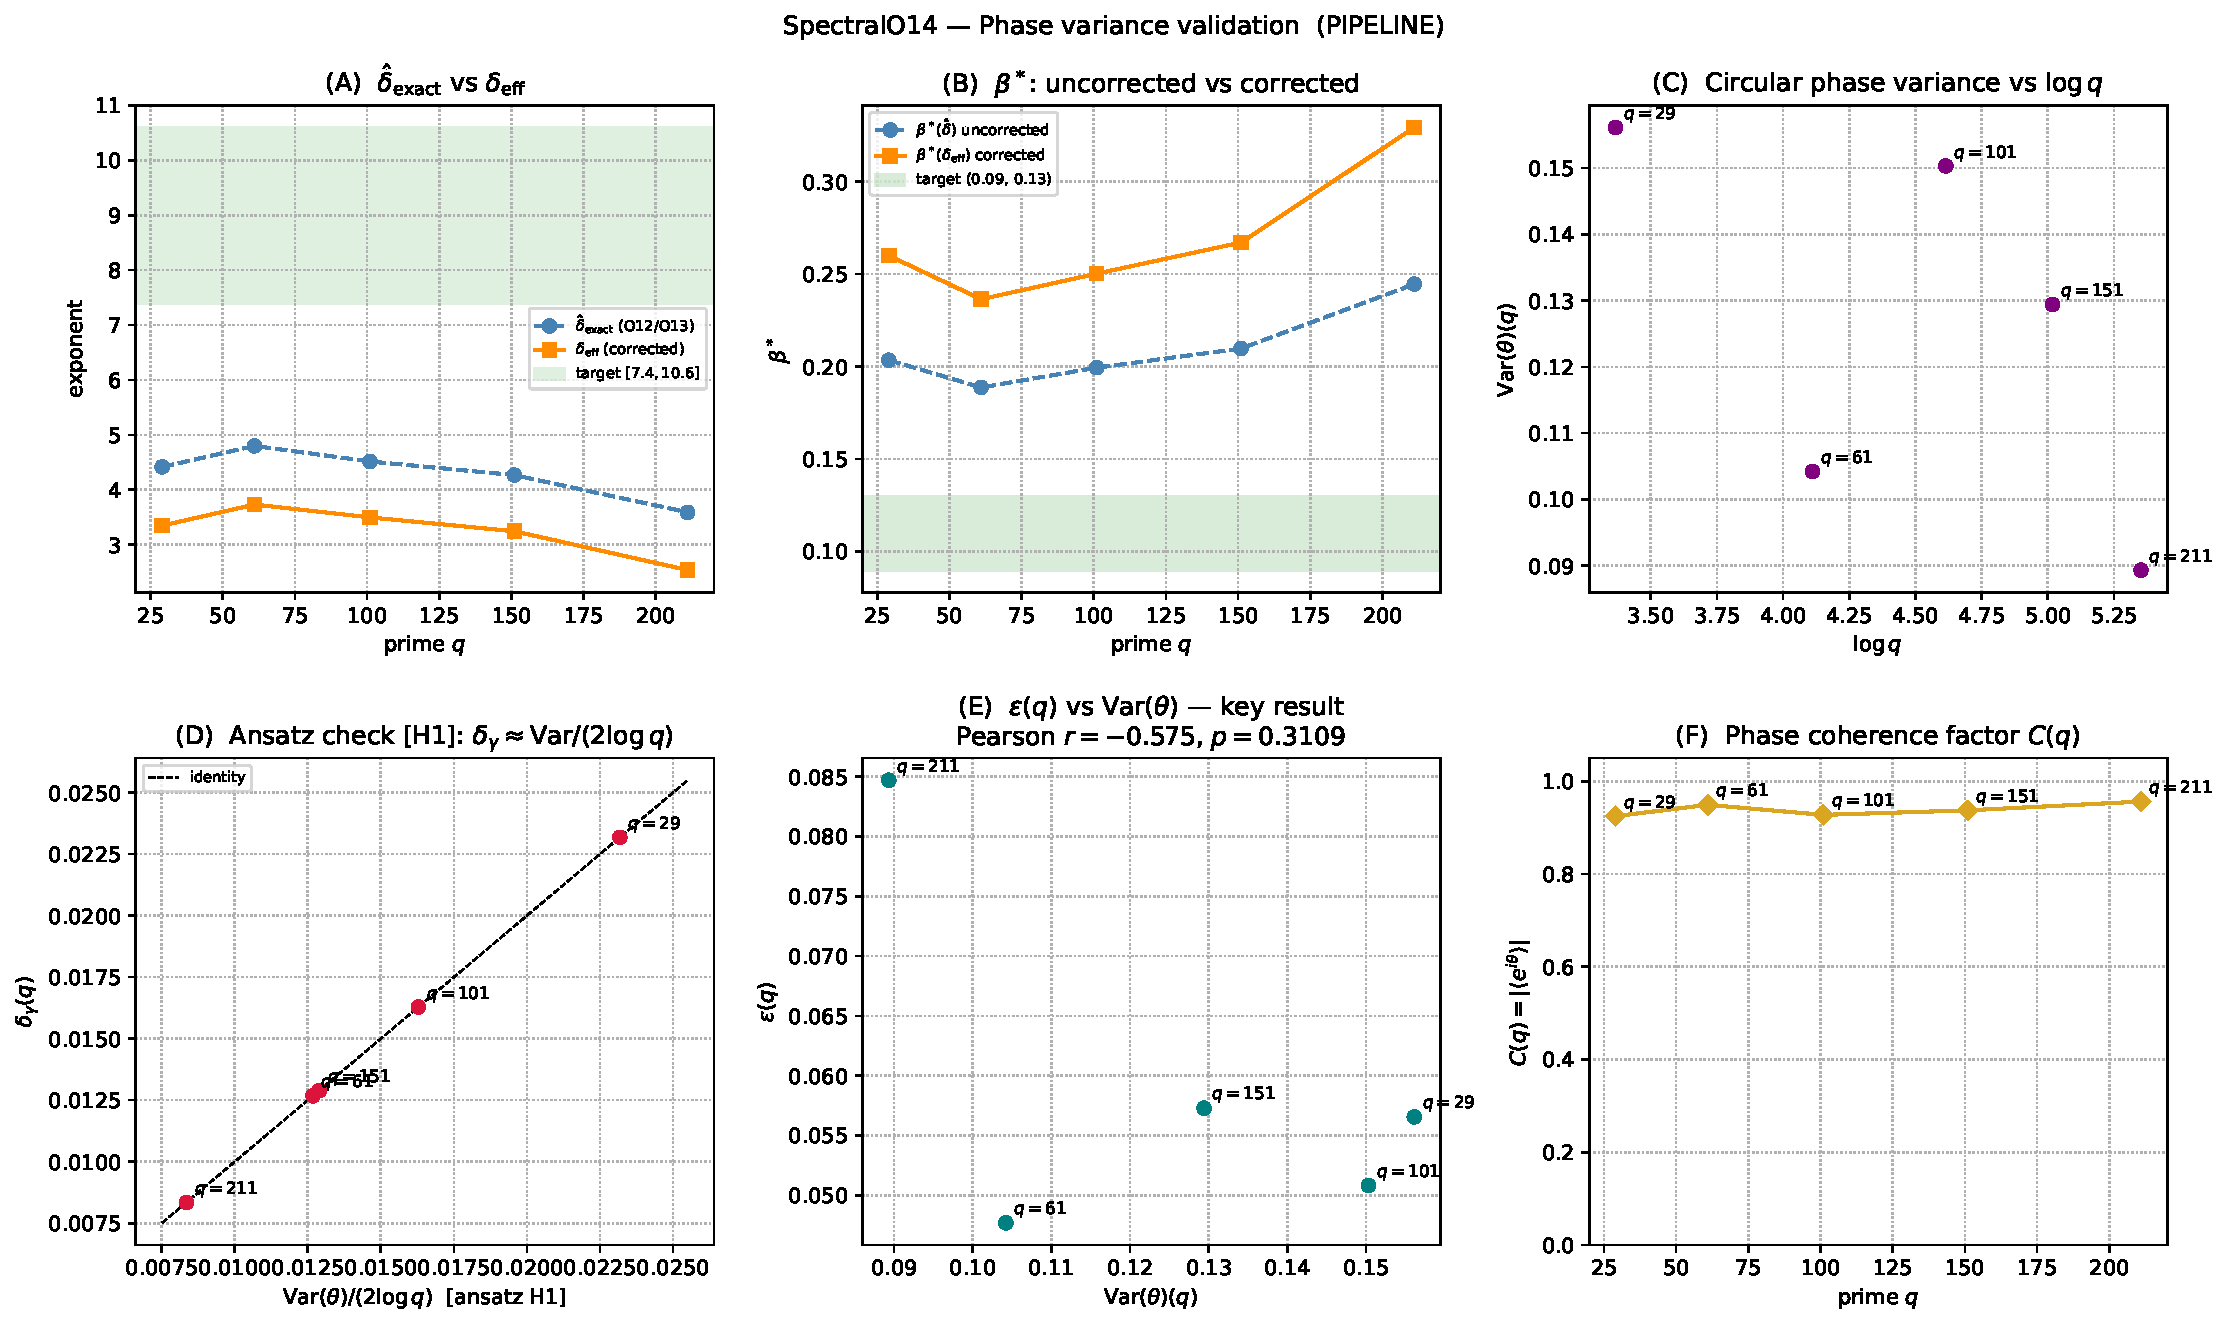
\includegraphics[width=\textwidth]{../code/fig_SpectralO14_validation}
    \caption{Conditional endpoint bookkeeping from the O12/O13 data.
      Panel~(A) displays the non-monotone finite-window slopes and the exact asymptotic exponent
      $\delta=3$.
      Panel~(B) compares those slopes with $\delta_{\mathrm{end}}$ under the benchmark $\eta=1/2$.
      Panel~(C) applies the imported reciprocal formula; all values remain outside the
      phenomenological interval $(0.09,0.13)$.
      Panel~(D) records the shell-level central-coordinate coherence as an independent null control,
      not as a contribution to rank.}
    \label{fig:validation}
  \end{figure}

  The endpoint term lies between $1.00$ and $1.06$, and
  $\delta_{\mathrm{end}}<5.0$ at every tested prime.
  This numerical fact selects S2-B inside the conditional diagnostic.
  The stronger transfer obstruction is independent of the table: the corpus supplies no native
  Heisenberg growth law implementing \eqref{eq:beta_delta}~\cite{Beau2026sgn}.

  \subsection{Two scenarios}
  \label{sec:scenarios}

  \paragraph{Scenario S2-A (phenomenological alignment).}
    If a specified inter-$q$ estimator stabilised above $7.0$, the imported reciprocal
    prescription would place $\beta_{\mathrm{diag}}$ in $(0.09,0.13)$.
    Such alignment would be numerical only; it would not construct a native Heisenberg
    capacity-to-rate bridge.

  \paragraph{Scenario S2-B (Structural revision).}
    The conditional endpoint diagnostic remains below $5.0$ in the pipeline data, so the
    observable-class bookkeeping does not close the numerical gap.
    The amplification mechanism of O3~\cite{Beau2026a7} would then require modification
    in the exact-block setting, or the link between mass ratios and spectral capacity would
    require a different structural interpretation.

  \section{Interpretive Consequences}
  \label{sec:physical}

  \subsection{Scenario S2-A: conditional alignment only}
    \label{sec:s2a}

    Even under S2-A, the observable-class mismatch would explain only the numerical tension inside
    the imported reciprocal prescription.
    It would not derive the cascade exponent from first principles.
    The generation structure established in SpectralStratigraphy~\cite{Beau2026a4} is unaffected
    by this distinction.

  \subsection{Scenario S2-B: required revisions}
    \label{sec:s2b}

    Under S2-B, at least one of the following modifications is required:
    \begin{enumerate}
      \item The amplification mechanism of O3~\cite{Beau2026a7} must be rederived in the exact-block
      setting, potentially yielding a different functional form for the
      $\delta \mapsto \beta^{*}$ map.
      \item The identification of $\beta^{*}$ with the charged-lepton cascade exponent requires
      reexamination, possibly via a sector-dependent exponent.
      \item The cross-substrate identification between Heisenberg capacity and the LPS rate variable
      must be supplied with a typed carrier and its own derivation.
    \end{enumerate}

  \subsection{Quark and neutrino sectors}
    \label{sec:quarks}

    Conditional use of \eqref{eq:beta_corrected} assigns a modelled term $\epsilon(q)$ depending
    on the block variance of the specific representation.
    Extension to the quark and neutrino sectors requires computing the block variance at the
    appropriate $q$ values for those sectors, which is left as open direction O14-O2
    (Section~\ref{sec:open}).

  \section{Open Directions}
  \label{sec:open}

  \paragraph{O14-O1 (Definition and normalisation of an inter-$q$ estimator).}
    Define an inter-$q$ estimator before assigning a normalisation exponent.
    The value $\eta=1/2$ is a numerical benchmark, not an intra-$q$ slope correction or a
    uniqueness theorem.
    A derivation requires an explicit estimator, a reason to normalise its amplitudes by a power of
    $q$, and a proof selecting that power without using the target value.

  \paragraph{O14-O2 (Quark and neutrino exponents).}
    The conditional diagnostic \eqref{eq:beta_corrected} may be evaluated for the block
    structures associated with the quark and neutrino representations.
    This requires identifying the appropriate Weil-block decomposition for those sectors and
    computing $\delta_{\mathrm{eff}}$ at the corresponding primes.

  \section{Conclusion}
  \label{sec:conclusion}

  The exact Weil-block observable and the proxy-level O7 prescription belong to different
  observable classes~\cite{Beau2026a11,Beau2026a16,Beau2026a17}.
  Two load-bearing gaps survive: the exact quantity is a mean over heterogeneous blocks, and no
  native Heisenberg growth carrier identifies that mean with the LPS rate variable.
  Projective-frequency overlap supplies the relevant within-block geometry.
  The central coordinate does not: it multiplies a Fourier mode by a non-zero scalar, so its
  contribution to every exact span rank and decay exponent is identically zero.

  The exact intra-$q$ result is Proposition~\ref{prop:fixed_q_invariance}: a factor
  $q^{-\eta}$ changes the intercept and cannot change the fitted decay exponent.
  The term $\eta\log q/\log n_1$ therefore belongs to an endpoint or inter-$q$ estimator whose
  full definition remains open.
  Equation~\eqref{eq:beta_corrected} is retained only as a phenomenological diagnostic under the
  imported LPS reciprocal prescription; it is not a native Heisenberg relation.

  The five finite-window slopes are non-monotone crossover statistics around the exact asymptotic
  exponent $\delta=3$.
  Under the explicit benchmark $\eta=1/2$, the sole displacement in the conditional endpoint
  diagnostic is $\eta\log q/\log n_1\approx1.00$--$1.06$.
  It does not alter the O12/O13 intra-$q$ slopes.
  The diagnostic remains below $5.0$ for all tested primes, selecting S2-B.

  O14 therefore supplies a partial intra-$q$ resolution of the observable-class mismatch and
  isolates the remaining estimator layer.
  It does not close the cross-substrate capacity-to-rate transfer, which is refuted as a native
  composite for the corpus-defined Heisenberg objects~\cite{Beau2026sgn}.

  \subsection*{Interpretive outlook}
  The exact capacity calculation measures how projective-frequency novelty is exhausted on a fixed
  Heisenberg graph.
  A particle-hierarchy rate is a different physical object.
  Their numerical proximity or separation cannot identify them.
  The constructive task is to provide a growth carrier, a typed map from capacity to that carrier's
  rate, and a selector for any cross-prime normalisation.
  Until those elements exist, the reciprocal formula is a conditional comparison tool rather than a
  prediction of the exact spectral pipeline.

  \bibliographystyle{plain}
      \bibliography{cosmochrony-bibliography}

\end{document}
